% !TEX encoding = UTF-8 Unicode
%%%%%%%%%%%%%%%%%%%%%%%%%%%%%%%%%%%%%%%%%
% Beamer Presentation
% LaTeX Template
% Version 1.0 (10/11/12)
%
% This template has been downloaded from:
% http://www.LaTeXTemplates.com
%
% License:
% CC BY-NC-SA 3.0 (http://creativecommons.org/licenses/by-nc-sa/3.0/)
%
%%%%%%%%%%%%%%%%%%%%%%%%%%%%%%%%%%%%%%%%%

%----------------------------------------------------------------------------------------
%	PACKAGES AND THEMES
%----------------------------------------------------------------------------------------

\documentclass{beamer}

\mode<presentation> {

% The Beamer class comes with a number of default slide themes
% which change the colors and layouts of slides. Below this is a list
% of all the themes, uncomment each in turn to see what they look like.

%\usetheme{default}
%\usetheme{AnnArbor}
%\usetheme{Antibes}
%\usetheme{Bergen}
%\usetheme{Berkeley}
%\usetheme{Berlin}
%\usetheme{Boadilla}
%\usetheme{CambridgeUS}
%\usetheme{Copenhagen}
%\usetheme{Darmstadt}
%\usetheme{Dresden}
%\usetheme{Frankfurt}
%\usetheme{Goettingen}
%\usetheme{Hannover}
%\usetheme{Ilmenau}
%\usetheme{JuanLesPins}
%\usetheme{Luebeck}
\usetheme{Madrid}
%\usetheme{Malmoe}
%\usetheme{Marburg}
%\usetheme{Montpellier}
%\usetheme{PaloAlto}
%\usetheme{Pittsburgh}
%\usetheme{Rochester}
%\usetheme{Singapore}
%\usetheme{Szeged}
%\usetheme{Warsaw}

% As well as themes, the Beamer class has a number of color themes
% for any slide theme. Uncomment each of these in turn to see how it
% changes the colors of your current slide theme.

%\usecolortheme{albatross}
%\usecolortheme{beaver}
%\usecolortheme{beetle}
%\usecolortheme{crane}
%\usecolortheme{dolphin}
%\usecolortheme{dove}
%\usecolortheme{fly}
%\usecolortheme{lily}
%\usecolortheme{orchid}
%\usecolortheme{rose}
%\usecolortheme{seagull}
%\usecolortheme{seahorse}
%\usecolortheme{whale}
%\usecolortheme{wolverine}

%\setbeamertemplate{footline} % To remove the footer line in all slides uncomment this line
%\setbeamertemplate{footline}[page number] % To replace the footer line in all slides with a simple slide count uncomment this line

%\setbeamertemplate{navigation symbols}{} % To remove the navigation symbols from the bottom of all slides uncomment this line
}

\usepackage{graphicx} % Allows including images
\usepackage{booktabs} % Allows the use of \toprule, \midrule and \bottomrule in tables
\usepackage{xeCJK}
\usepackage{color}
\usepackage{listings}
\usepackage{tikz}
\usepackage{multirow}
\lstset{numbers=left,xleftmargin=10pt,xrightmargin=10pt}

%----------------------------------------------------------------------------------------
%	TITLE PAGE
%----------------------------------------------------------------------------------------

\title[EL\&JSTL]{EL\&JSTL} % The short title appears at the bottom of every slide, the full title is only on the title page

\author{张海宁} % Your name
\institute[gzu] % Your institution as it will appear on the bottom of every slide, may be shorthand to save space
{
贵州大学 \\ % Your institution for the title page
\medskip
\textit{hnzhang1@gzu.edu.cn} % Your email address
}
\date{\today} % Date, can be changed to a custom date

\begin{document}

\begin{frame}
\titlepage % Print the title page as the first slide
\end{frame}

\begin{frame}
\frametitle{Overview} % Table of contents slide, comment this block out to remove it
\tableofcontents % Throughout your presentation, if you choose to use \section{} and \subsection{} commands, these will automatically be printed on this slide as an overview of your presentation
\end{frame}

%----------------------------------------------------------------------------------------
%	PRESENTATION SLIDES
%----------------------------------------------------------------------------------------

%------------------------------------------------
\section{EL} % Sections can be created in order to organize your presentation into discrete blocks, all sections and subsections are automatically printed in the table of contents as an overview of the talk
%------------------------------------------------
\begin{frame}
\Huge{\centerline{EL}}
\end{frame}
\begin{frame}
\frametitle{什么是EL}
EL是指jsp \textcolor{red}{E}xpression \textcolor{red}{L}anguage。EL是jsp2.0引入的,其目的就是为了简化jsp页面中的的一些参数获取操作(using html like tags)。\\

使用EL可以方便的读取存储在以下对象中的数据:
\begin{itemize}
\item
JavaBean
\item
jsp的一些内置对象
\begin{itemize}
\item
request
\item
session
\item
application
\item
...
\end{itemize}
\end{itemize}
\begin{block}{语法结构}
\$\{ expression \}
\end{block}
\end{frame}
\begin{frame}{EL的隐含对象}
\label{elimplicit}
与jsp的内置对象(参考本ppt第\ref{implicitobj},\ref{scope}页)类似的概念,可以直接使用。
EL的隐含对象可以分为以下三类:
\begin{itemize}
\item
页面上下文对象
\item
访问作用域范围的隐含对象
\item
访问环境信息的隐含对象
\end{itemize}
\end{frame}
\begin{frame}[fragile]{页面上下文对象}
\begin{block}{}
\begin{lstlisting}
${pageContext.request }
<% request.getMethod(); %>
${pageContext.request.method }

${pageContext.response }
${pageContext.out }
${pageContext.session }
${pageContext.page }

\end{lstlisting}
\end{block}
\end{frame}

\begin{frame}[fragile]{访问作用域范围的隐含对象}
\begin{block}{}
\begin{lstlisting}
<%
pageContext.setAttribute("university", "pgGzu", 1);
request.setAttribute("university", "reqGzu");
session.setAttribute("university", "sessionGzu");
application.setAttribute("university", "appGzu");
%>
${pageScope.university }
${requestScope.university }
${sessionScope.university }
${applicationScope.university }
${university }
\end{lstlisting}
\end{block}
结合\${university},来看作用域的查找顺序:
page$>$request$>$session$>$application
\end{frame}

\begin{frame}[fragile]{访问环境信息的隐含对象}
\begin{block}{}
\begin{lstlisting}
${param.course }
<%request.getParameter("course"); %>
<!--获取复选框的值  -->
${paramValues.multiCheckBox[0] }
${paramValues.multiCheckBox[1] }

${header.connection }
${header["connection"] }
${header["User-Agent"] }

${cookie.JSESSIONID }
${cookie.JSESSIONID.value }
\end{lstlisting}
\end{block}
\end{frame}
%\begin{frame}
%\begin{table}
%\begin{tabular}{ll}
%\toprule
%\textbf{Impicit Objects}&\textbf{Usage}\\
%\midrule
%pageScope&访问page scope范围内的属性\\
%requestScope&访问request scope范围内的属性\\
%sessionScope&访问session scope范围内的属性\\
%applicationScope&访问application scope范围内的属性\\
%param&访问request parameter\\
%paramValues&访问request parameter的名称\\
%header&访问header范围内的属性\\
%headerValues&返回header范围内的属性名称\\
%cookie&访问cookie范围内的属性\\
%initParam&访问initParam\\
%pageContext&访问pageContext范围内的属性\\

%\bottomrule
%\end{tabular}
%\caption{Implicit Objects in EL}
%\end{table}
%\end{frame}
\begin{frame}[fragile]
\frametitle{param示例}
\begin{block}{the form in test.jsp}
\begin{lstlisting}
<form action="showCookie.jsp" method="post">
课程:<select name="course">
<option  value="AnalogCircuit" >模电</option>
...
</select>
备注:<input name="note" type="text">
<button type="submit">submit</button>
</form>
\end{lstlisting}
\end{block}
\textcolor{red}{Question: }怎么在showCookie.jsp页面获取数据?
\end{frame}
\begin{frame}[fragile]
\frametitle{param示例}
\begin{block}{get the form parameter of test.jsp in showCookie.jsp}
\begin{lstlisting}
The course is: ${param.course}.
\end{lstlisting}
\end{block}
\textcolor{red}{Question: }怎么在showCookie.jsp页面获取cookie相关的数据?
\end{frame}
\begin{frame}{EL的操作符}
与jsp的内置对象类似的概念,可以直接使用。
\begin{table}
\begin{tabular}{lp{9em}ll}
\toprule
\textbf{Operator}&\textbf{Description}&\textbf{Operator}&\textbf{Description}\\
\midrule
.&访问bean里的属性或map里的记录&\\
$[]$&访问array或list里的元素&()&改变优先级\\
+ - * /&+ - * /&\%&取余\\
==(eq)&判断是否相等&!=(nq)&判断是否不相等\\
$<$(lt)&判断是否小于&$>$(gt)&判断是否大于\\
$<=$(le)&判断是否小于或相等&$>=$(ge)&判断是否大于或相等\\
\&\&(and)&与&||(or)&或\\
!(not)&非&empty&判断是否为空\\

\bottomrule
\end{tabular}
\caption{Basic Operators in EL}
\end{table}
\end{frame}

\section{JSTL}
\begin{frame}
\Huge{\centerline{JSTL}}
\end{frame}
\begin{frame}
\frametitle{什么是JSTL}
JSTL是\textcolor{red}{J}avaServer Pages \textcolor{red}{S}tandard \textcolor{red}{T}ag \textcolor{red}{L}ibrary (JSTL)的简称。JSTL提供了一系列封装好了的jsp标签,可以取代在jsp页面中嵌入java代码的做法。

JSTL实际上由5个功能不同的标签库组成:

\begin{enumerate}
\item
\textcolor{red}{核心标签库}
\item
格式标签库
\item
SQL标签库
\item
XML标签库
\item
函数标签库
\end{enumerate}

\end{frame}
\begin{frame}
\frametitle{核心标签库}
核心标签库主要用于完成JSP页面的常用功能,包括:
\begin{itemize}
\item
表达式标签
\begin{itemize}
\item
$<c:out>, <c:set>, <c:remove>, <c:catch>$
\end{itemize}
\item
URL标签
\begin{itemize}
\item
$<c:import>, <c:redirect>, <c:url>, <c:param>$
\end{itemize}
\item
流程控制标签
\begin{itemize}
\item
$<c:if>, <c:choose>, <c:when>, <c:otherwise>$
\end{itemize}
\item
循环控制标签
\begin{itemize}
\item
$<c:forEach>, <c:forTokens>$
\end{itemize}
\end{itemize}
\end{frame}
\begin{frame}{核心标签库中各标签的作用}
\begin{table}
\begin{tabular}{p{10em}l}
\toprule
\textbf{tag}&\textbf{Description}\\
\midrule
$<c:out>$&将表达式的值输出到jsp页面\\
$<c:set>$&在指定的作用域内定义变量或为变量赋值\\
$<c:remove>$&从指定的作用域中移除指定的变量\\
$<c:catch>$&捕获程序的异常\\
$<c:import>$&导入文件到web页面中\\
$<c:redirect>$&将request请求重定向到其他URL\\
$<c:url>$&构造一个URL\\
$<c:param>$&为其他标签提供参数信息\\
$<c:if>$&简单的条件判断\\
$<c:choose>, <c:when>, <c:otherwise>$&选择,相当于switch\\
$<c:forEach>$&遍例数组或集合类中的成员\\
$<c:forTokens>$&迭代字符串中由分隔符分隔的成员\\
\bottomrule
\end{tabular}
%\caption{JSTL核心标签库中标签的作用}
\end{table}
\end{frame}
\begin{frame}[fragile]
\frametitle{JSTL的配置}
\begin{enumerate}
\item
下载JSTL的jar文件

\url{http://tomcat.apache.org/download-taglibs.cgi#Standard-1.2.5}
\item
将下载好的taglibs-standard-impl-1.2.5.jar文件,放到项目下的WEB-INF文件夹下的lib文件夹中
\item
在想使用JSTL标签的jsp页面中,定义引用的标签库和访问前缀
\begin{lstlisting}
<%@ taglib prefix = "c" 
  uri = "http://java.sun.com/jsp/jstl/core" %>
\end{lstlisting}
\end{enumerate}
\end{frame}

\begin{frame}
\frametitle{表达式标签<c:out>}
<c:out>标签用于将表达式的值输出到jsp页面中去。类似于jsp的<\%=exp\%>或el的\$\{exp\}。

\textcolor{red}{<c:out value="" [escapeXml="true|false"]  [default="defaultValue"] />}
\begin{itemize}
\item
value

用于指定变量或表达式,可以使用el
\item
escapeXml

可选属性,默认为true,转换。用于指定是否转换value中的特殊字符。比如将<转换为\&lt;
\item
default

可选属性,默认为空字符串。用于指定当value的值为null时,将要显示的默认值。
\end{itemize}
\textcolor{red}{<c:out value="<br>newline" />} 这里<br>原样输出 

\textcolor{red}{ <c:out value="<br>newline" escapeXml="false"/>}这里<br>会被解析为html标记
\end{frame}
\begin{frame}[fragile]
\frametitle{完成Reg里的doPost()方法-II}
\begin{lstlisting}
protected void doPost(... , ...)... {
// 设置request传递过来值的编码,并获取传递值
//get current date and time
//write to database
int i = db.writeDb("teachers", fields, values);
db.getClose();
String rz="";
if(i==1) {
  rz = "Done! Will return  in 3 seconds.";
}else {
  rz = "Sth wrong! Will return  in 3 seconds.";
}
response.getWriter().print(rz);
response.setHeader("refresh","3,URL=teacher.jsp");
}
\end{lstlisting}
\end{frame}

\begin{frame}{servlet过滤器}
先观察下图:
\begin{figure}
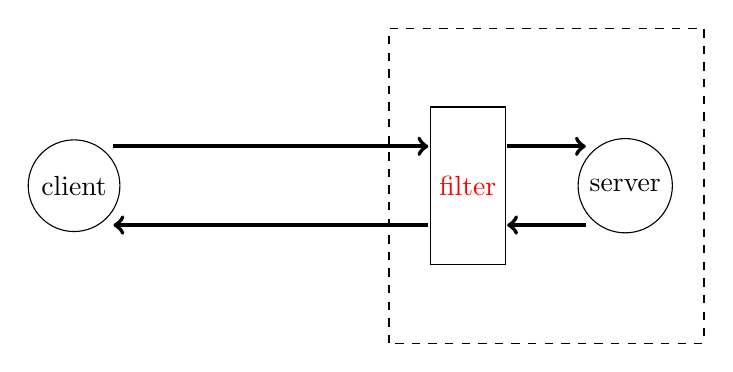
\begin{tikzpicture}
\node (c) at (1,5) [circle,draw] {client};

\node (f) at (6,5) [rectangle,draw,minimum height=20mm] {\textcolor{red}{filter}};
\node (s) at (8,5) [circle,draw] {server};
\draw [dashed,label=above:webserver] (5,3) rectangle (9,7) ;
\draw [->,line width=1.5pt] (1.5,5.5) -- (5.5,5.5); 
\draw [<-,line width=1.5pt] (1.5,4.5) -- (5.5,4.5); 
\draw [->,line width=1.5pt] (6.5,5.5) -- (7.5,5.5); 
\draw [<-,line width=1.5pt] (6.5,4.5) -- (7.5,4.5); 

\end{tikzpicture}
\caption{the position and function of a filter}
\end{figure}
可以看出,filter是介于client和server端的一个“关卡”,其负责“过滤”信息流(这个过滤器可以有多个,形成过滤器链)。
\end{frame}
\begin{frame}[fragile]{创建一个filter}
创建一个filter,禁止特定id的用户注册(\textcolor{red}{chain.doFilter()})。

创建过程与创建servlet类似。

FilterReg.java的主要代码如下所示:
\begin{lstlisting}
@WebFilter(filterName = "/FilterReg",
      urlPatterns = "/Reg")
public class FilterReg implements Filter {
  public void doFilter(ServletRequest request, 
  ServletResponse response, FilterChain chain)  {
  HttpServletRequest req = 
      (HttpServletRequest) request; 
  String id = request.getParameter("staffid");
  System.out.println("staffid is: "+id);
  // pass the request along the filter chain
  chain.doFilter(request, response);
  }
}
\end{lstlisting}
\end{frame}
\begin{frame}[fragile]{chain.doFilter()}
Pay attention to 
\textcolor{red}{chain.doFilter()}.
\begin{lstlisting}
public void doFilter(ServletRequest request, 
    ServletResponse response, FilterChain chain){
HttpServletRequest req = 
  (HttpServletRequest) request; 
String id = request.getParameter("staffid");
System.out.println("staffid is: "+id);
	
// pass the request along the filter chain
chain.doFilter(request, response);
		
HttpServletResponse resp = 
    (HttpServletResponse) response;
resp.getWriter().print("add is done. Stay here.");
//resp.setHeader("refresh", "3,URL=index.jsp");
}
\end{lstlisting}
\end{frame}

\begin{frame}{监听器}
\textcolor{red}{监听}是对\textcolor{red}{特定事件}进行关注。

所谓监听器就是对特定事件的发生做出反应,比如你点击了什么按钮等等。
\begin{table}
\begin{tabular}{ll}
\toprule
\textbf{Listener接口}&\textbf{Event类}\\
\midrule
ServletContextListener&ServletContextEvent\\
ServletContexAttributeListener&ServletContextAttributeEvent\\
HttpSessionListener&\multirow{2}{*}{HttpSeesionEvent}\\
HttpSessionActivationListener&\\
HttpSessionAttributeListener&\multirow{2}{*}{HttpSessionBindingEvent}\\
HttpSessionBindingListener&\\
ServletRequestListener&ServletRequestEvent\\
ServletRequestAttributeListener&ServletRequestAttributeEvent\\
\bottomrule
\end{tabular}
\caption{Listener接口与Event类}
\end{table}
\end{frame}


\begin{frame}[fragile]{使用servlet处理文件上传I}
form的主要代码为(class\_apply.jsp):
\begin{lstlisting}
<form action="ServletClassArrange" 
  enctype="multipart/form-data" method="post">
<table>
<tr><td>
上传实验指导书:<input type="file" name="guideBook" >
   </td></tr>
<tr><td>
<button type="submit">submit</button>
   </td></tr>
</table>
</form>
\end{lstlisting}
\end{frame}
\begin{frame}[fragile]{使用servlet处理文件上传II}
Servlet的主要代码为(ServletClassArrange.java):
\begin{lstlisting}
@WebServlet("/ServletClassArrange")
@MultipartConfig
public class ServletClassArrange 
   extends HttpServlet {
 protected void doPost(......){
  request.setCharacterEncoding("utf-8");
  Part pt = request.getPart("guideBook");
  String fName = pt.getSubmittedFileName();
  System.out.println("the file is:"+fName);
  System.out.println(
   this.getServletContext().getRealPath("/")+fName);
  pt.write("/Users/hainingzhang/Downloads/"+fName);
  System.out.println("success uploaded!");
 }
}
\end{lstlisting}
\end{frame}
%---------------------------------------------
\section{数据库分页}
\begin{frame}
\Huge{\centerline{javabean}}
\end{frame}
\begin{frame}{什么是javabean}
如果一个类满足以下条件:
\begin{enumerate}
\item
All properties private (use getters/setters)
\item
A public no-argument constructor
\item
Implements Serializable
\end{enumerate}
则就称这个类是一个javabean。
\end{frame}
\begin{frame}[fragile]{serializable}
如果想将一个java对象保存到文件中,那么这个对象必须是可序列化的(serializable),也就是说这个对象的类需要是可序列化的。
\begin{block}{Teacher类实现序列化}
\begin{lstlisting}
import java.io.Serializable;

public class Teacher implements Serializable{
   private static final long serialVersionUID = 1L;
}
\end{lstlisting}
\end{block}
\end{frame}
\begin{frame}{为什么要使用javabean}
使用javabean可以使html代码和java代码尽可能的分离,将java代码单独封装成为一个处理某种业务逻辑的类,然后在jsp页面中调用此类。以\textcolor{red}{简化jsp页面和提高java程序代码的重用性}。
\end{frame}
\begin{frame}[fragile]{Teacher}
定义Teacher类,该类为封装教师对象的javabean。
\begin{lstlisting}
//Teacher.java
package bean;
import java.io.Serializable;
public class Teacher implements Serializable{
 private static final long serialVersionUID = 1L;
 private String staffid,nm,logDate;	
 public Teacher() {}
 public void setstaffid(String id){this.staffid=id;}
 public void setnm(String name) {this.nm=name;}
 public void setlogDate(String logDate) {
   this.logDate=logDate;}
 public String getstaffid() { return staffid; }
 public String getnm() { return nm;  }
 public String getlogDate() { return logDate;  }
}
\end{lstlisting}

\end{frame}
\begin{frame}[fragile]{与javabean相关的几个jsp标签}
\begin{enumerate}
\item
jsp:useBean

实例化一个对象
\item
jsp:setProperty

为一个属性赋值
\item
jsp:getProperty

获取一个属性值
\end{enumerate}
\begin{lstlisting}
//teacher_add.jsp
<jsp:useBean id="teacher" class="bean.Teacher">
 </jsp:useBean>
<jsp:setProperty name="teacher" property="nm"
 value="贵州大学" />
<jsp:getProperty property="nm" name="teacher"/>

\end{lstlisting}

\end{frame}

\begin{frame}[fragile]{对javabean属性赋值与获取javabean属性}
在jsp页面中,对javabean属性赋值与获取javabean属性。
\begin{lstlisting}
//teacher_add.jsp
<% request.setCharacterEncoding("utf-8"); %>
<jsp:useBean id="teacher" class="bean.Teacher">
 </jsp:useBean>
<jsp:setProperty name="teacher" property="*" />
<table>  <tr> <th>staffid</th> <th>nm</th> 
      <th>logDate</th> </tr>  <tr> <td>
<jsp:getProperty property="staffid" name="teacher"/>
</td><td>
<jsp:getProperty property="nm" name="teacher"/>
</td><td>
<jsp:getProperty property="logDate" name="teacher"/>
</td></tr></table>
\end{lstlisting}

\end{frame}

\begin{frame}{作业}
\begin{enumerate}
\item
使用session记录登陆状态
\item
练习servlet和javabean的使用
\item
学习jsp+servlet+javabean联合使用

\url{https://github.com/danielniko/SimpleJspServletDB}
\end{enumerate}
\end{frame}
%------------------------------------------------

\begin{frame}
\Huge{\centerline{The End}}
\end{frame}

%---------------------------------------
\section{Appendix}

\begin{frame}
\Huge{\centerline{Appendix}}
\end{frame}

\subsection{JSP 9个内置对象}
\begin{frame}{内置对象}
\label{implicitobj}
\begin{table}
\begin{tabular}{lll}
\toprule
\textbf{Object}&\textbf{Description}&\textbf{Scope}\\
\midrule
request&封装了客户端请求&\\
response&封装了服务器端的回应信息&\\
out&向response中写数据&\\
session&保存一次会话的信息&一次会话\\
application&保存应用程序中的公有数据&系统的全局变量\\
config&&ServletConfig\\
pageContext&获取jsp页面上下文,进而获取内置对象&\\
page&调用当前jsp页面中的变量或方法&this的同意词\\
exception&用来处理异常信息的&\\
\bottomrule
\end{tabular}
\caption{implicit objects of jsp}

\end{table}
返回\ref{elimplicit}
\end{frame}
\subsection{JSP 4个作用域}
\begin{frame}{作用域}
\begin{table}
\label{scope}
\begin{tabular}{ll}
\toprule
\textbf{Scope}&\textbf{Description}\\
\midrule
page&当前的页面\\
request&当前的请求\\
session&当前的会话\\
application&当前网站\\
\bottomrule
\end{tabular}
\caption{scopes of jsp}
\end{table}
返回\ref{elimplicit}
\end{frame}
\subsection{相关资源}
\begin{frame}
\begin{block}{ppt、项目源代码及实验指导书的地址}
\begin{enumerate}
\item
ppt

\url{https://github.com/gmsft/ppt/tree/master/javaweb}
\item
lab-java项目

\url{https://github.com/gmsft/javaweb}

\item
实验指导书

暂无,拟放在ppt的仓库里
\end{enumerate}
\end{block}
\end{frame}



%----------------------------------------------------------------------------------------

\end{document} 